\chapter{Vertauschbare Observablen, Energiephasen und Spinpräzession}

\lectureoverview{Wir beginnen mit der qualitativen Bedeutung der Unschärfe. Zwei Observablen können nur dann gleichzeitig scharfe Werte haben, wenn sie eine vollständige gemeinsame Eigenbasis besitzen; dies ist gleichbedeutend damit, dass ihre Operatoren kommutieren. Anschließend wiederholen wir die unitäre Zeitentwicklung und die Schr\"odinger-Gleichung, vergleichen Kommutatoren mit klassischen Poisson-Klammern, lösen die zeitabhängige Gleichung in der Energiebasis und wenden das Ergebnis auf einen Spin in einem Magnetfeld an. Die abschließende Rechnung ergibt die Präzession der Erwartungswerte des Spins, die zwei Energieniveaus eines allgemeinen Spin-Hamiltonoperators und den Unterschied zwischen einem seitlichen Erwartungswert und einem Photon mit der halben Energielücke.}

Der Spin mit zwei Zuständen bleibt unser einfachstes Quantensystem. Ein Hilbert-Raum mit drei Zuständen wäre die nächsteinfachere abstrakte Möglichkeit; zwei Spins haben bereits vier orthogonale Basiszustände. Zwei Spins fügen wir noch nicht zusammen, obwohl dieser Schritt naheliegt und Verschränkung mit sich bringen wird. Zunächst sollten wir das Ein-Spin-Problem abschließen und die Vorstellungen von Unschärfe und Zeitentwicklung auf eine solidere Grundlage stellen.

\section{Wann zwei Größen gleichzeitig scharf sein können}

Eine gute Messung ist wiederholbar. Wird eine Observable gemessen und der Wert \(l\) erhalten, sollte eine unmittelbar anschließende Wiederholung denselben Wert ergeben. Die erste Messung muss das System daher zumindest vorübergehend in einem Eigenzustand des zugehörigen Operators zurücklassen:
\begin{equation}
L\ket{l}=l\ket{l}.
\end{equation}
Diese operationale Aussage genügt, um den qualitativen Ursprung der Unschärfe sichtbar zu machen.

Angenommen, zwei Observablen \(L\) und \(M\) lassen sich gleichzeitig messen. Eine gemeinsame Messung muss beide angegebenen Werte scharf lassen. Die möglichen Zustände nach der Messung müssen folglich gleichzeitige Eigenvektoren beider Operatoren sein. In dem hier betrachteten endlichdimensionalen Fall können wir eine vollständige orthonormale Menge \(\{\ket{i}\}\) wählen, die
\begin{equation}
L\ket{i}=l_i\ket{i},
\qquad
M\ket{i}=m_i\ket{i}.
\label{eq:l5-common-eigenvectors}
\end{equation} erfüllt.

\begin{remark}Mit dem Wort \emph{Basis} ist eine vollständige orthonormale Basis gemeint. Die lineare Algebra erlaubt auch nichtorthogonale Basen, doch für Quantenzustände ist die orthonormale Konvention besonders natürlich. Entartete Eigenwerte lassen innerhalb eines Eigenraums einen Spielraum; die Eigenvektoren können in diesem Raum orthonormal gewählt werden.
\end{remark}

\begin{theorem}Zwei endlichdimensionale hermitesche Observablen sind genau dann gleichzeitig messbar, wenn sie eine vollständige gemeinsame Eigenbasis besitzen, was gleichbedeutend damit ist, dass sie kommutieren.
\end{theorem}

Die eine Richtung folgt unmittelbar aus Gleichung~\eqref{eq:l5-common-eigenvectors}. Wirkt man in der einen Reihenfolge, ergibt sich
\begin{align}
ML\ket{i}
&=M\bigl(l_i\ket{i}\bigr)\\
&=l_i m_i\ket{i},
\end{align}
In umgekehrter Reihenfolge ergibt sich dagegen
\begin{align}
LM\ket{i}
&=L\bigl(m_i\ket{i}\bigr)\\
&=m_i l_i\ket{i}.
\end{align}
Die Eigenwerte sind gewöhnliche Zahlen, also gilt \(l_i m_i=m_i l_i\). Daher wirken \(ML\) und \(LM\) auf jedes Element einer Basis und somit auf jeden Zustand gleich:
\begin{equation}
[L,M]\equiv LM-ML=0.
\label{eq:l5-commuting-condition}
\end{equation}

\begin{figure}[htbp]\centering
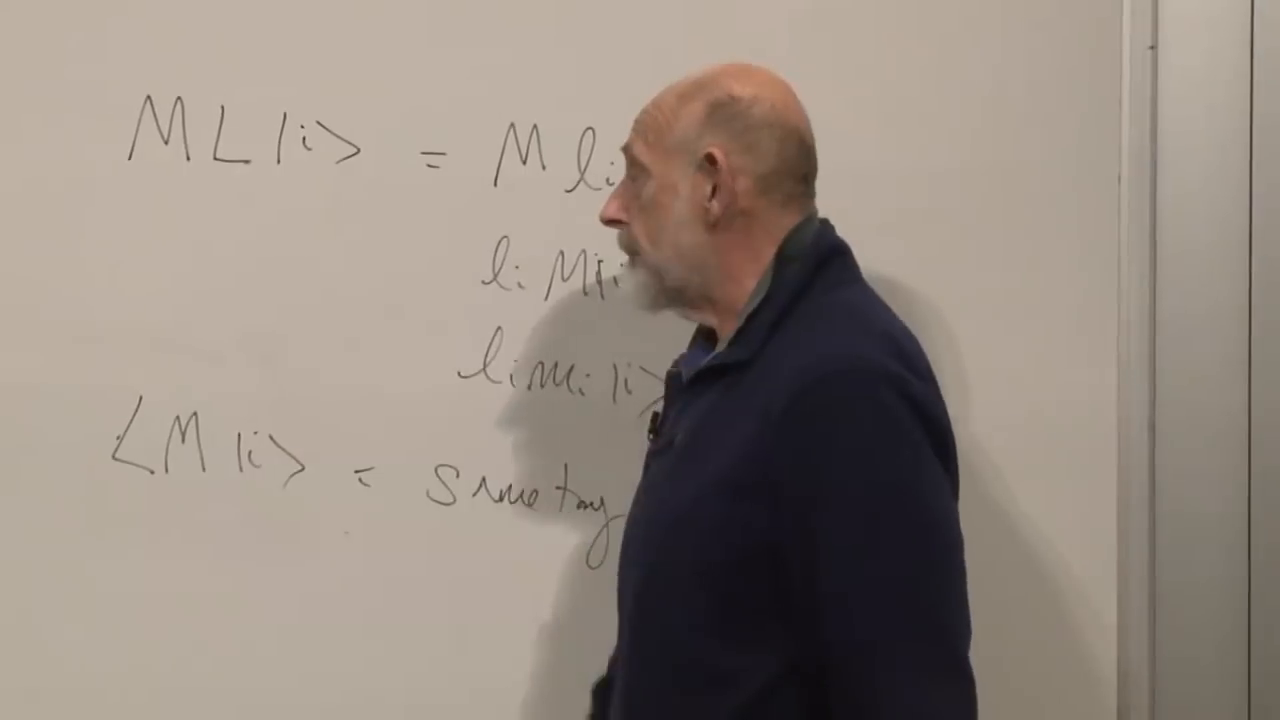
\includegraphics[width=0.86\textwidth]{lecture_05_figure_02.png}\caption{Das Argument mit gemeinsamen Eigenvektoren führt zu \(LM-ML=[L,M]=0\).}\lectureframe{00:10:30}\end{figure}

Auch die Umkehrung gilt: Kommutierende hermitesche Operatoren lassen sich simultan diagonalisieren. Hat ein Operator einen entarteten Eigenraum, so bildet der andere diesen Eigenraum auf sich selbst ab und lässt sich darin diagonalisieren. Wiederholt man dies in jedem Eigenraum, erhält man eine vollständige gemeinsame Eigenbasis.

Die Pauli-Operatoren liefern das erste wichtige Gegenbeispiel. Je zwei der Operatoren \(\sigma_x,\sigma_y,\sigma_z\) kommutieren nicht. Die Eigenzustände von \(\sigma_z\) sind Spin-aufwärts und Spin-abwärts, während diejenigen von \(\sigma_x\) rechts und links sind. Man kann eine der beiden Komponenten scharf präparieren und ihre Messung wiederholen, aber nicht beide Komponenten zugleich scharf präparieren. Das ist Unschärfe, noch bevor irgendeine numerische Ungleichung eingeführt wurde.

Später werden wir quantifizieren, wie die Unschärfen zweier nichtkommutierender Observablen einander beschränken. Hier wird kein numerisches Unschärfeprinzip bewiesen. Der entscheidende Punkt geht der Ungleichung voraus: Nichtkommutativität verhindert, dass ein Zustand beiden Größen zugleich scharfe Werte zuordnet.

\begin{classroomqa}\audiencequestion{Warum erfordert eine gemeinsame Messung gemeinsame Eigenvektoren?}\lecturerresponse{Eine wiederholbare Messung hinterlässt einen Zustand, in dem der gemessene Wert scharf ist; das bedeutet, dass der Zustand ein Eigenzustand des gemessenen Operators ist. Werden zwei Werte zugleich bestimmt und bleiben beide Messungen wiederholbar, muss der resultierende Zustand ein Eigenzustand beider Operatoren sein. Die vollständige Menge der gemeinsamen Messergebnisse liefert daher eine gemeinsame Eigenbasis.}\end{classroomqa}

\begin{classroomqa}\audiencequestion{Geht es dabei um zwei verschiedene Teilchen?}\lecturerresponse{Das muss nicht sein, denn \(\sigma_x\) und \(\sigma_z\) wirken bereits auf einen einzelnen Spin. Bei zwei verschiedenen Teilsystemen kommutieren Observablen, die auf unterschiedliche Faktoren wirken, jedoch miteinander: \(A\otimes I\) kommutiert mit \(I\otimes B\). Deshalb lassen sich eine Komponente des einen Spins und eine Komponente des anderen zugleich messen. Die Zusammensetzung solcher Systeme wird später zur Verschränkung führen.}\end{classroomqa}

\section{Unitäre Zeitentwicklung und ihr Generator}

Die Definition eines Zustands hat in der Quantenmechanik erheblich länger gedauert als in der klassischen Mechanik. Ist der Zustandsraum jedoch einmal festgelegt, ist die Bewegungsgleichung kompakt. Es gelte
\begin{equation}
\ket{\psi(t)}=U(t)\ket{\psi(0)}.
\label{eq:l5-propagator}
\end{equation}
Die Zeitentwicklung muss die Unterscheidbarkeit erhalten. Mehr noch: Sie erhält alle Skalarprodukte. Für eine orthonormale Basis gilt
\begin{equation}
\bra{j}U^\dagger(t)U(t)\ket{i}=\delta_{ji},
\end{equation}
und somit
\begin{equation}
U^\dagger(t)U(t)=I.
\label{eq:l5-unitarity}
\end{equation}
Der Zeitentwicklungsoperator ist unitär.

Bei verschwindender verstrichener Zeit gilt \(U(0)=I\). Stetigkeit bedeutet dann, dass sich die Entwicklung während eines kleinen Zeitintervalls \(\epsilon\) nur wenig von der Identität unterscheidet. In Einheiten mit \(\hbar=1\) schreiben wir
\begin{equation}
U(\epsilon)=I-i\epsilon H+O(\epsilon^2),
\qquad
U^\dagger(\epsilon)=I+i\epsilon H^\dagger+O(\epsilon^2).
\end{equation}
Einsetzen in Gleichung~\eqref{eq:l5-unitarity} ergibt
\begin{equation}
H^\dagger=H.
\end{equation}
Der Generator der Zeitentwicklung ist hermitesch und daher eine Observable. Er ist der Hamiltonoperator.

Wendet man den infinitesimalen Zeitentwicklungsoperator auf einen Zustand an, erhält man
\begin{equation}
\ket{\psi(\epsilon)}
=\ket{\psi(0)}-i\epsilon H\ket{\psi(0)}+O(\epsilon^2).
\end{equation}
Umstellen ergibt den an der Tafel notierten Differenzenquotienten:
\begin{equation}
\frac{\ket{\psi(\epsilon)}-\ket{\psi(0)}}{\epsilon}
=-iH\ket{\psi(0)}+O(\epsilon).
\end{equation}

\begin{figure}[htbp]\centering
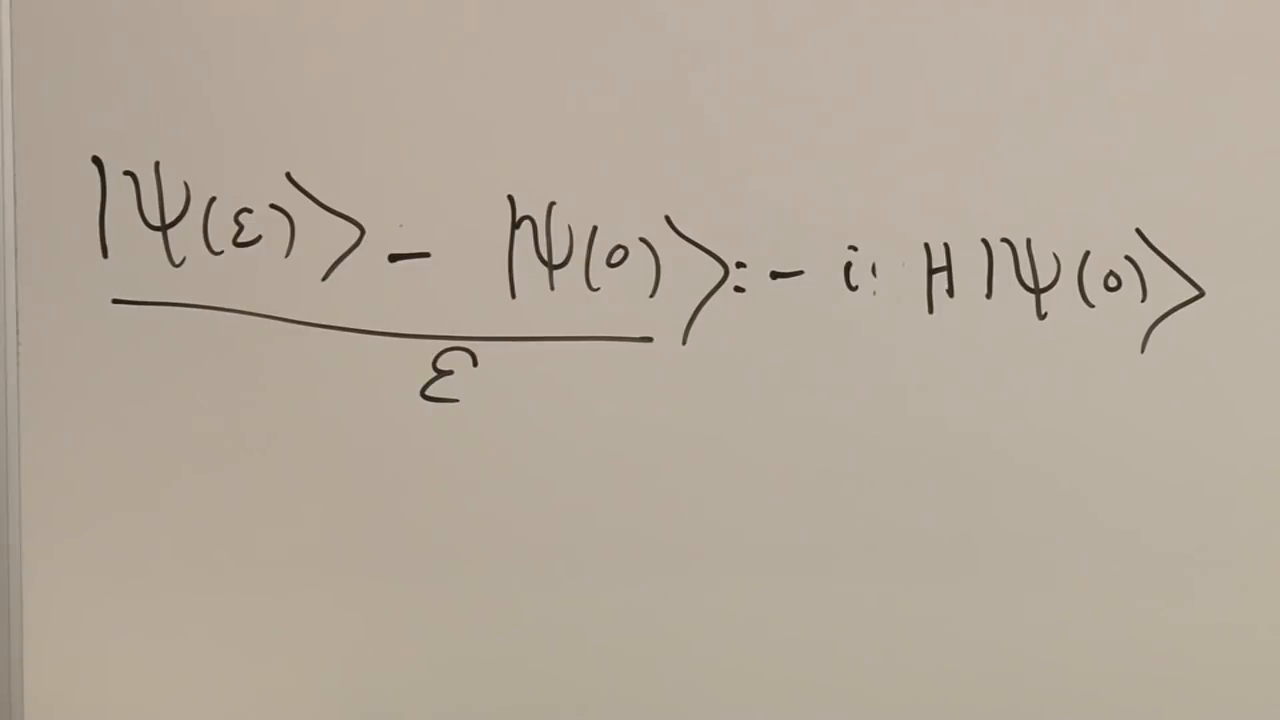
\includegraphics[width=0.86\textwidth]{lecture_05_figure_03.png}\caption{Die infinitesimale Zustandsänderung als Differenzenquotient.}\lectureframe{00:23:33}\end{figure}

Im Grenzübergang \(\epsilon\to0\) erhalten wir die zeitabhängige Schr\"odinger-Gleichung:
\begin{equation}
\frac{d}{dt}\ket{\psi(t)}=-iH\ket{\psi(t)}.
\label{eq:l5-schrodinger}
\end{equation}
Mit wieder eingesetzten Konstanten lautet sie \(i\hbar\,d\ket{\psi}/dt=H\ket{\psi}\).

Schr\"odingers ursprüngliche Gleichung bezog sich auf die Wellenfunktion eines bewegten Teilchens. Die obige Operatorgleichung wurde einst verallgemeinerte Schr\"odinger-Gleichung genannt, weil sie gleichermaßen für einen Spin, ein System mit drei Zuständen, zwei Spins oder ein System beliebiger Komplexität gilt. Das Adjektiv wird heute meist weggelassen; dies ist inzwischen einfach die allgemeine Form der Gleichung.

Gleichung~\eqref{eq:l5-schrodinger} legt die Entwicklung des Zustands eindeutig fest, solange das System ungestört bleibt. Dadurch werden nicht alle Messergebnisse eindeutig. Ein Quantenzustand legt Wahrscheinlichkeiten für mögliche Messungen fest, und die Gleichung entwickelt diese Wahrscheinlichkeiten über die sich ändernden Amplituden fort. Eine Messung verändert den Zustand im Allgemeinen und unterbricht diese isolierte Entwicklung.

\begin{classroomqa}\audiencequestion{Stört jede Messung das System?}\lecturerresponse{Im Allgemeinen ja, aber es gibt einen wichtigen Sonderfall. Ist der Zustand bereits ein Eigenzustand der Observable, kann eine ideale wiederholbare Messung ihren Wert bestätigen, ohne den Zustand zu verändern. Im Allgemeinen ist es nicht möglich, eine beliebige Observable zu messen, ohne andere, inkompatible Eigenschaften zu stören.}\end{classroomqa}

\section{Energie und die zeitunabhängige Gleichung}

Da \(H\) hermitesch ist, sind seine Eigenwerte reell und seine Eigenvektoren können zu einer vollständigen orthonormalen Basis gewählt werden:
\begin{equation}
H\ket{E_i}=E_i\ket{E_i}.
\label{eq:l5-time-independent}
\end{equation}
Dies ist die zeitunabhängige Form der Schr\"odinger-Gleichung. Sie ist ein Eigenwertproblem und keine Bewegungsgleichung: Gefragt wird, welche Energiewerte das System annehmen kann und in welchen Zuständen diese Werte scharf sind.

Das Spektrum hängt vom System ab. Gebundene Atombewegungen und der harmonische Oszillator haben abzählbare Energieniveaus. Ein ungebundenes Teilchen kann ein kontinuierliches Spektrum besitzen. Energie lässt sich auf vielerlei Weise messen; im Prinzip könnte man sogar eine hinreichend präzise Massenmessung über \(E=mc^2\) verwenden, obwohl dies in der Praxis selten die geeignete Methode ist. Ein reales System besitzt bereits seinen Hamiltonoperator; die Physikerin oder der Physiker legt ihn nicht fest, sondern versucht, ihn zu bestimmen. Ist dieser Operator bekannt, besteht die mathematische Aufgabe darin, seine Eigenwerte und Eigenvektoren zu finden.

Addiert man eine Konstante \(cI\) zu \(H\), verschiebt sich jede Energie um \(c\). Der gesamte Zustand wird dabei mit einer gemeinsamen Phase \(e^{-ict}\) multipliziert, was weder Wahrscheinlichkeiten noch Erwartungswerte ändert. Für die hier betrachtete Dynamik sind nur Energiedifferenzen relevant.

\section{Zeitentwicklung der Erwartungswerte}

Der geläufige Ausdruck \emph{Erwartungswert} bezeichnet einen statistischen Mittelwert. Für eine Observable \(L\) gilt
\begin{equation}
\expect{L}(t)=\bra{\psi(t)}L\ket{\psi(t)}.
\end{equation}
In diesem Schritt tragen nur die Zustandsvektoren eine Zeitabhängigkeit. Leitet man beide Seiten ab und verwendet Gleichung~\eqref{eq:l5-schrodinger} sowie deren hermitesch konjugierte Gleichung,
\begin{equation}
\frac{d}{dt}\ket{\psi}=-iH\ket{\psi},
\qquad
\frac{d}{dt}\bra{\psi}=i\bra{\psi}H,
\end{equation}
erhält man
\begin{align}
\frac{d}{dt}\expect{L}
&=i\bra{\psi}HL\ket{\psi}
  -i\bra{\psi}LH\ket{\psi}\\
&=-i\expect{[L,H]}.
\label{eq:l5-expectation-motion}
\end{align}

\begin{figure}[htbp]\centering
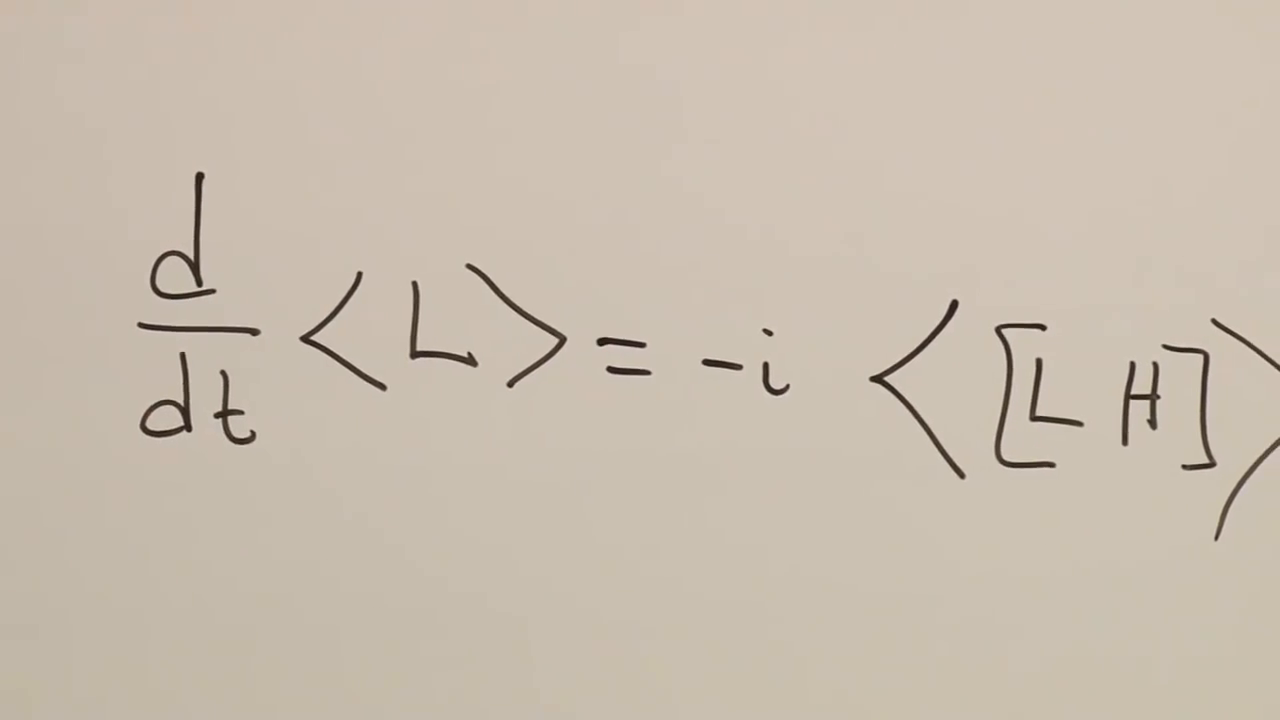
\includegraphics[width=0.86\textwidth]{lecture_05_figure_04.png}\caption{Die Bewegungsgleichung für den Erwartungswert in Kommutatorform.}\lectureframe{00:35:35}\end{figure}

Der Faktor \(i\) stellt die Realität von \(\expect{L}\) nicht infrage. Für hermitesche Operatoren \(L\) und \(H\) ist der Kommutator antihermitesch:
\begin{equation}
[L,H]^\dagger=-[L,H].
\end{equation}
Sein Erwartungswert ist daher rein imaginär, sodass die Multiplikation mit \(-i\) eine reelle Ableitung ergibt.

Man verwendet gelegentlich die Kurzschreibweise
\begin{equation}
\dot L=-i[L,H].
\end{equation}
An dieser Stelle ist sie als Abkürzung für Gleichung~\eqref{eq:l5-expectation-motion} zu lesen, also als Gleichung über Mittelwerte. Eine vollständige Änderung des Bildes, in der die Operatoren selbst die Zeitabhängigkeit tragen, folgt später.

\subsection{Die Algebra der Kommutatoren}

Kommutatoren sind antisymmetrisch:
\begin{equation}
[A,B]=-[B,A].
\end{equation}
Außerdem erfüllen sie eine Produktregel, die der Leibnizregel für Ableitungen ähnelt:
\begin{equation}
[AB,C]=A[B,C]+[A,C]B.
\label{eq:l5-product-rule}
\end{equation}
Zur Überprüfung behalten wir die Reihenfolge aller Faktoren bei:
\begin{align}
A[B,C]+[A,C]B
&=A(BC-CB)\\
&\quad +(AC-CA)B\\
&=ABC-ACB\\
&\quad +ACB-CAB\\
&=ABC-CAB\\
&=[AB,C].
\end{align}

\begin{figure}[htbp]\centering
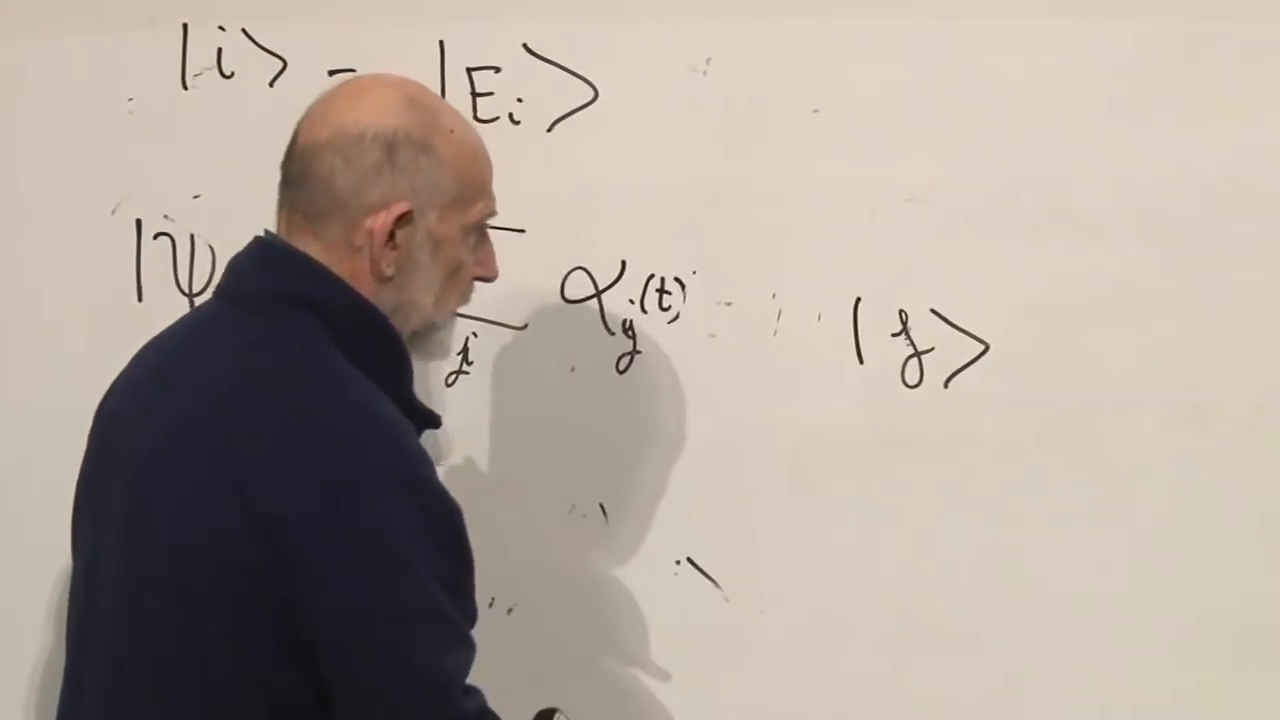
\includegraphics[width=0.86\textwidth]{lecture_05_figure_05.png}\caption{Überprüfung der Produktregel für Kommutatoren durch Ausmultiplizieren beider Seiten.}\lectureframe{00:43:10}\end{figure}

\begin{classroomqa}\audiencequestion{Wird die linke Seite durch die rechte Seite der Produktregel versehentlich doppelt gezählt?}\lecturerresponse{Nein. Beim Ausmultiplizieren erhält man die beiden gesuchten Terme \(ABC\) und \(-CAB\). Die beiden hinzugefügten Terme sind \(-ACB\) und \(+ACB\); sie heben sich genau auf. Die scheinbare zusätzliche Kopie ist der Zwischenterm, der benötigt wird, um den Ausdruck auf die beiden verlangten Arten zu faktorisieren.}\end{classroomqa}

Dieselbe Antisymmetrie und Produktregel gelten für klassische Poisson-Klammern. Diese strukturelle Ähnlichkeit ist kein Zufall. Die klassische Entsprechung lautet
\begin{equation}
\{A,B\}
\quad\longleftrightarrow\quad
\frac{1}{i\hbar}[A,B]
=-\frac{i}{\hbar}[A,B].
\label{eq:l5-poisson-correspondence}
\end{equation}
In Einheiten mit \(\hbar=1\) hat die klassische Gleichung
\begin{equation}
\frac{dL}{dt}=\{L,H\}
\end{equation}
dieselbe Form wie Gleichung~\eqref{eq:l5-expectation-motion}. In gewöhnlichen makroskopischen Einheiten ist \(\hbar\) winzig, und Kommutatoren werden im geeigneten klassischen Grenzfall vernachlässigbar. Dies ist die wesentliche Konsistenzprüfung, die den quantenmechanischen Generator \(H\) mit dem Hamiltonoperator der klassischen Mechanik identifiziert.

Der Faktor \(\hbar\) ist aus Dimensionsgründen erforderlich. Eine Poisson-Klammer differenziert nach konjugierten Koordinaten und Impulsen, während ein Operator-Kommutator direkt aus Produkten gebildet wird. Das Plancksche Wirkungsquantum stellt die Umrechnung zwischen diesen Dimensionen bereit.

Setzen wir \(L=H\). Da jeder Operator mit sich selbst kommutiert, gilt
\begin{equation}
\frac{d}{dt}\expect{H}
=-i\expect{[H,H]}=0.
\end{equation}
Für die hier betrachteten zeitunabhängigen Hamiltonoperatoren ist der mittlere Energiewert erhalten. Eine stärkere Aussage über die gesamte Energieverteilung ist möglich, aber hier genügt der Mittelwert.

\begin{classroomqa}\audiencequestion{Wofür steht \(L\) in diesen Gleichungen? Ist es der Drehimpuls?}\lecturerresponse{Hier bezeichnet \(L\) einen allgemeinen hermiteschen linearen Operator, also eine beliebige Observable. Es kann sich um eine Spin-Komponente, einen Ort oder sogar um \(H\) selbst handeln. Der Buchstabe steht für \emph{linearen Operator} und ist nicht als Drehimpuls zu verstehen, solange diese Bedeutung nicht ausdrücklich angegeben ist.}\end{classroomqa}

\begin{classroomqa}\audiencequestion{Warum führt der Faktor \(i\) nicht dazu, dass sich für einen reellen Mittelwert eine imaginäre Ableitung ergibt?}\lecturerresponse{Der Kommutator zweier hermitescher Operatoren ist antihermitesch, daher ist sein Erwartungswert imaginär. Die nachfolgende Rechnung mit den Pauli-Matrizen macht dies konkret: Ihre Kommutatoren enthalten einen expliziten Faktor \(2i\), der den Faktor \(-i\) in der Bewegungsgleichung aufhebt.}\end{classroomqa}

\section{Lösen der Schr\"odinger-Gleichung in der Energiebasis}

Nehmen wir an, das Energieeigenwertproblem sei gelöst. Entwickeln wir einen beliebigen Zustand in der festen Energiebasis:
\begin{equation}
\ket{\psi(t)}=\sum_j\alpha_j(t)\ket{E_j}.
\label{eq:l5-energy-expansion}
\end{equation}
In dieser Darstellung ändern sich die Basisvektoren nicht; die gesamte Zeitabhängigkeit steckt in den Koeffizienten. Setzt man Gleichung~\eqref{eq:l5-energy-expansion} in Gleichung~\eqref{eq:l5-schrodinger} ein, erhält man
\begin{align}
\sum_j\dot\alpha_j(t)\ket{E_j}
&=-i\sum_j\alpha_j(t)H\ket{E_j}\\
&=-i\sum_j E_j\alpha_j(t)\ket{E_j}.
\end{align}
Aus der Eindeutigkeit der Entwicklung nach einer Basis folgt für jedes feste \(j\):
\begin{equation}
\dot\alpha_j(t)=-iE_j\alpha_j(t),
\qquad\text{no sum on \(j\)}.
\end{equation}
Die Lösung lautet
\begin{equation}
\alpha_j(t)=\alpha_j(0)e^{-iE_jt}.
\label{eq:l5-energy-phase}
\end{equation}

\begin{figure}[htbp]\centering
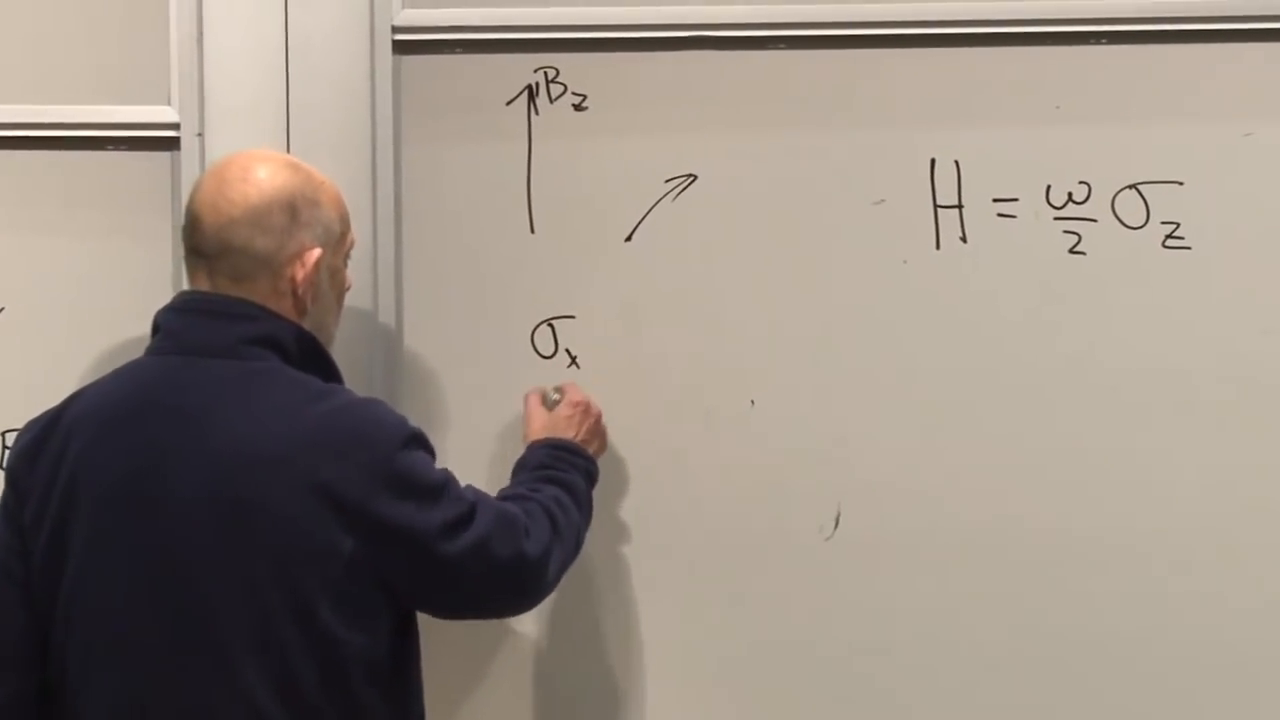
\includegraphics[width=0.86\textwidth]{lecture_05_figure_06.png}\caption{Für jeden Koeffizienten in der Energiebasis gilt eine eigene Exponentialgleichung für die Phase.}\lectureframe{01:03:25}\end{figure}

Die allgemeine Lösung lautet somit
\begin{equation}
\ket{\psi(t)}
=\sum_j\alpha_j(0)e^{-iE_jt}\ket{E_j}.
\label{eq:l5-general-solution}
\end{equation}
Setzt man die Einheiten wieder ein, wird \(E_jt\) durch \(E_jt/\hbar\) ersetzt. Der Betrag jedes Koeffizienten bleibt unverändert:
\begin{equation}
|\alpha_j(t)|=|\alpha_j(0)|.
\end{equation}
Die Zeitentwicklung ändert die relativen Phasen. Ein einzelner Energieeigenzustand erhält nur eine gemeinsame Phase und hat daher zeitunabhängige Messwahrscheinlichkeiten.

Der Erwartungswert von \(L\) lässt sich nun explizit angeben. Wir definieren seine Matrixelemente in der Energiebasis durch
\begin{equation}
L_{kj}=\bra{E_k}L\ket{E_j}.
\end{equation}
Dann gilt
\begin{align}
\expect{L}(t)
&=\sum_{k,j}
\alpha_k^*(0)\alpha_j(0)
e^{i(E_k-E_j)t}
L_{kj}.
\label{eq:l5-heisenberg-matrix}
\end{align}

\begin{figure}[htbp]\centering
\includegraphics[width=0.86\textwidth]{lecture_05_figure_07.png}\caption{Die Matrixformel in der Energiebasis: Jeder Eintrag trägt eine Phase mit der Übergangsfrequenz.}\lectureframe{01:10:45}\end{figure}

Die Diagonalterme \(k=j\) sind konstant. Ein Nebendiagonalelement oszilliert mit der Energiedifferenz \(E_k-E_j\). Der hier dargestellten historischen Einordnung zufolge erkannte Heisenberg diese Matrixstruktur, bevor die moderne Herleitung mit Zustandsvektoren verfügbar war; Diracs Notation machte ihre Bedeutung später transparent.

\begin{classroomqa}\audiencequestion{Bleiben die Beträge der Koeffizienten \(\alpha_j\) konstant?}\lecturerresponse{Ja. Jeder Koeffizient wird mit einer komplexen Phase vom Betrag eins multipliziert. Nur die relativen Phasen ändern sich, und durch sie können sich Erwartungswerte mit Nebendiagonalelementen zeitlich verändern.}\end{classroomqa}

\begin{classroomqa}\audiencequestion{Sollte die Schr\"odinger-Gleichung eine partielle oder eine totale Ableitung enthalten?}\lecturerresponse{Beim hier verwendeten abstrakten Zustand \(\ket{\psi(t)}\) ist die Zeit die einzige angegebene Variable; daher haben beide Schreibweisen denselben Inhalt. Später wird eine Wellenfunktion wie \(\psi(x,t)\) sowohl vom Ort als auch von der Zeit abhängen. Dann ist die Schreibweise mit partieller Ableitung naheliegend.}\end{classroomqa}

\begin{classroomqa}\audiencequestion{Ist die Erhaltung der Orthogonalität lediglich eine empirische Annahme?}\lecturerresponse{Sie wird durch Experimente gestützt, ist aber zugleich ungewöhnlich restriktiv. Versuche, die unitäre Quantenmechanik zu deformieren, zerstören tendenziell die Positivität oder die Wahrscheinlichkeitserhaltung, die kausale Lokalität oder die konsistente Behandlung zusammengesetzter Systeme. David Finkelstein beschrieb deformierbare Theorien als solche, die plastisch fließen, und starre Theorien als solche, die spröde brechen. In diesem Sinne ist die Quantenmechanik spröde: Beliebige kleine Änderungen führen normalerweise nicht zu einer benachbarten konsistenten Theorie.}\end{classroomqa}

\begin{classroomqa}\audiencequestion{Warum sind die Energieeigenwerte \(E_j\) reell?}\lecturerresponse{Die Unitarität impliziert, dass der infinitesimale Generator \(H\) hermitesch ist; jeder Eigenwert eines hermiteschen Operators ist reell. Die Schlusskette lautet also: Erhaltung der Orthogonalität, Unitarität, Hermitizität von \(H\) und schließlich Realität des Energiespektrums.}\end{classroomqa}

\section{Ein Spin in einem Magnetfeld}

Welcher Hamiltonoperator ist einem einzelnen Spin zuzuordnen? Ein isolierter Spin im ansonsten leeren Raum hat keine ausgezeichnete Richtung und daher keinen nichttrivialen Hamiltonoperator: Dieser ist proportional zur Einheitsmatrix und bewirkt keine beobachtbare Bewegung. Ein Magnetfeld liefert sowohl eine Wechselwirkungsenergie als auch eine Achse.

Wir richten das Feld entlang \(z\) aus. Ein geladenes Teilchen mit Spin besitzt ein magnetisches Moment, und die bekannte Dipolenergie ist proportional zur Ausrichtung dieses Moments relativ zum Feld. Feldstärke, magnetisches Moment, Vorzeichenkonvention und \(\hbar\) fassen wir in der Konstanten \(\omega\) zusammen:
\begin{equation}
H=\frac{\omega}{2}\sigma_z.
\label{eq:l5-z-hamiltonian}
\end{equation}
Der Faktor \(1/2\) ist zweckmäßig, weil die Kommutatoren der Pauli-Matrizen einen Faktor \(2\) enthalten.

Das klassische Pfeilbild muss mit Vorsicht verwendet werden. Ein quantenmechanischer Spin besitzt keine zugleich scharfen Komponenten \(x\), \(y\) und \(z\); daher kann kein gewöhnlicher Pfeil alle seine Eigenschaften gleichzeitig darstellen. Die nützliche dreidimensionale Größe wird der Vektor der Erwartungswerte sein, nicht der zweikomponentige Zustandsvektor selbst.

\subsection{Pauli-Kommutatoren}

Wir verwenden die Matrixdarstellungen
\begin{equation}
\begin{aligned}
\sigma_x&=
\begin{pmatrix}0&1\\1&0\end{pmatrix},\\[0.4em]
\sigma_y&=
\begin{pmatrix}0&-i\\i&0\end{pmatrix},\\[0.4em]
\sigma_z&=
\begin{pmatrix}1&0\\0&-1\end{pmatrix}.
\end{aligned}
\end{equation}
Zum Beispiel gilt
\begin{align}
[\sigma_z,\sigma_x]
&=
\begin{pmatrix}1&0\\0&-1\end{pmatrix}
\begin{pmatrix}0&1\\1&0\end{pmatrix}
-
\begin{pmatrix}0&1\\1&0\end{pmatrix}
\begin{pmatrix}1&0\\0&-1\end{pmatrix}\\
&=
\begin{pmatrix}0&1\\-1&0\end{pmatrix}
-
\begin{pmatrix}0&-1\\1&0\end{pmatrix}\\
&=2
\begin{pmatrix}0&1\\-1&0\end{pmatrix}
=2i\sigma_y.
\end{align}
Die zyklischen Beziehungen lauten
\begin{equation}
\begin{aligned}
[\sigma_z,\sigma_x]&=2i\sigma_y,\\
[\sigma_x,\sigma_y]&=2i\sigma_z,\\
[\sigma_y,\sigma_z]&=2i\sigma_x.
\end{aligned}
\label{eq:l5-pauli-commutators}
\end{equation}
Vertauscht man die beiden Einträge, wechselt das Vorzeichen.

\begin{figure}[htbp]\centering
\includegraphics[width=0.86\textwidth]{lecture_05_figure_08.png}\caption{Die drei Pauli-Kommutatoren schließen sich zyklisch auf den Pauli-Matrizen selbst.}\lectureframe{01:33:30}\end{figure}

Diese Beziehungen haben dieselbe zyklische Struktur wie die klassischen Poisson-Klammern des Drehimpulses. Außerdem schließen sie sich auf den ursprünglichen drei Operatoren, wodurch die Bewegungsgleichungen besonders einfach werden.

\begin{classroomqa}\audiencequestion{Müssen die Kommutatoren mit Bra-Ket-Klammern berechnet werden?}\lecturerresponse{Nein. Operatorprodukte werden durch Matrixprodukte dargestellt, daher ermöglichen die \(2\times2\)-Matrizen eine bequeme direkte Rechnung. Alternativ könnte man die Operatoren nacheinander auf die Basiszustände Spin-aufwärts und Spin-abwärts anwenden und erhielte dasselbe Ergebnis.}\end{classroomqa}

\subsection{Präzession der Erwartungswerte}

Wir wenden Gleichung~\eqref{eq:l5-expectation-motion} mit dem Hamiltonoperator aus Gleichung~\eqref{eq:l5-z-hamiltonian} an:
\begin{align}
\frac{d}{dt}\expect{\sigma_x}
&=-i\frac{\omega}{2}\expect{[\sigma_x,\sigma_z]}
=-\omega\expect{\sigma_y},\\
\frac{d}{dt}\expect{\sigma_y}
&=-i\frac{\omega}{2}\expect{[\sigma_y,\sigma_z]}
=+\omega\expect{\sigma_x},\\
\frac{d}{dt}\expect{\sigma_z}
&=-i\frac{\omega}{2}\expect{[\sigma_z,\sigma_z]}
=0.
\label{eq:l5-spin-motion}
\end{align}

\begin{figure}[htbp]\centering
\begin{minipage}[c]{0.62\textwidth}\centering
\includegraphics[width=\textwidth]{lecture_05_figure_09.png}\end{minipage}\hfill
\begin{minipage}[c]{0.31\textwidth}\centering
\begin{tikzpicture}[scale=0.78,>=Latex]
  \draw[->,thick] (0,0) -- (0,3.0) node[above] {\(z\parallel\bm B\)};
  \draw[dashed] (0,1.8) ellipse (1.45 and 0.42);
  \draw[->,very thick] (0,0) -- (1.05,1.8)
    node[right] {\(\expect{\bm\sigma}\)};
  \draw[->,thick] (1.38,1.67)
    arc[start angle=-12,end angle=245,x radius=1.45,y radius=0.42];
\end{tikzpicture}\end{minipage}\caption{Die Gleichungen an der Tafel und ihre geometrische Konsequenz: Die transversalen Erwartungswerte rotieren, während die feldparallele Komponente konstant bleibt. Der Pfeil stellt die drei Erwartungswerte dar, keinen verborgenen klassischen Spin.}\lectureframe{01:35:28}\end{figure}

Die ersten beiden Gleichungen beschreiben eine Kreisbewegung in der transversalen Ebene:
\begin{align}
\expect{\sigma_x}(t)
&=\expect{\sigma_x}(0)\cos\omega t
-\expect{\sigma_y}(0)\sin\omega t,\\
\expect{\sigma_y}(t)
&=\expect{\sigma_x}(0)\sin\omega t
+\expect{\sigma_y}(0)\cos\omega t.
\end{align}
Unterdessen bleibt \(\expect{\sigma_z}\) konstant. Der Vektor der Erwartungswerte präzediert daher mit der Kreisfrequenz \(\omega\) um die Magnetfeldachse.

Die Operatoren in dieser Rechnung im Schr\"odinger-Bild sind feste Matrizen. Der Zustand ändert sich, und damit vollführen die Mittelwerte die bekannte Kreiselbewegung.

\begin{classroomqa}\audiencequestion{Wie kann ein zweidimensionaler Zustandsraum ein dreidimensionales Präzessionsbild hervorbringen?}\lecturerresponse{Der Zustandsvektor hat bis auf Normierung und Gesamtphase zwei komplexe Komponenten. Der dargestellte Vektor im dreidimensionalen Raum ist dagegen \(\bigl(\expect{\sigma_x},\expect{\sigma_y},\expect{\sigma_z}\bigr)\). Diese Erwartungswerte werden durch den Zustand bestimmt und bilden das Bild des Bloch-Vektors, sind aber nicht selbst der Zustandsvektor.}\end{classroomqa}

\section{Der allgemeinste Hamiltonoperator für einen einzelnen Spin}

Jede hermitesche \(2\times2\)-Matrix lässt sich entwickeln als
\begin{equation}
H=aI+b_x\sigma_x+b_y\sigma_y+b_z\sigma_z,
\end{equation}
mit reellen Koeffizienten. Der Einheitsanteil ändert nur die Gesamtphase. Die drei übrigen Koeffizienten lassen sich als Komponenten eines Vektors auffassen. Bezeichnen wir seinen Betrag mit \(\omega/2\) und seine Richtung mit dem Einheitsvektor \(\bm n\), so lautet der nichttriviale Hamiltonoperator
\begin{equation}
H=\frac{\omega}{2}\,\bm\sigma\cdot\bm n,
\qquad
\bm\sigma\cdot\bm n
=n_x\sigma_x+n_y\sigma_y+n_z\sigma_z.
\label{eq:l5-general-spin-h}
\end{equation}
Für \(\bm B=B\bm n\) gibt \(\bm n\) die Feldrichtung an, während \(\omega\) zusammen mit der magnetischen Kopplung die Feldstärke festlegt. Die Orientierung wird durch \(\bm n\) angegeben, nicht durch \(\omega\).

Die Bewegungsgleichung nimmt die kompakte Form an
\begin{equation}
\frac{d}{dt}\expect{\bm\sigma}
=\omega\,\bm n\times\expect{\bm\sigma}.
\end{equation}
Die Komponente entlang \(\bm n\) kommutiert mit \(H\) und bleibt konstant; die senkrechten Komponenten präzedieren um \(\bm n\).

\begin{classroomqa}\audiencequestion{Warum ist dies die richtige Form des Hamiltonoperators?}\lecturerresponse{Es gibt nur vier linear unabhängige hermitesche \(2\times2\)-Matrizen: \(I,\sigma_x,\sigma_y,\sigma_z\). Der Einheitsanteil bewirkt bei einem einzelnen Spin keine beobachtbare Bewegung. Daher ist jeder nichttriviale zeitunabhängige Hamiltonoperator eines einzelnen Spins eine reelle Linearkombination der drei Pauli-Matrizen. Ein Magnetfeld fasst diese drei Koeffizienten in einem Betrag und einer Richtung zusammen.}\end{classroomqa}

\begin{classroomqa}\audiencequestion{Wofür steht \(\omega\) genau?}\lecturerresponse{Es ist eine skalare Größe, die proportional zum Betrag des Feldes mal dem magnetischen Moment ist; konventionelle Konstanten sind darin bereits enthalten. Sie legt sowohl die Präzessionsfrequenz als auch die Energieaufspaltung fest. Der Einheitsvektor \(\bm n\) gibt die Feldrichtung an.}\end{classroomqa}

\subsection{Die beiden Energieniveaus}

Schreiben wir Gleichung~\eqref{eq:l5-general-spin-h} in Matrixform, so ergibt sich
\begin{equation}
\bm\sigma\cdot\bm n
=
\begin{pmatrix}
n_z & n_x-in_y\\
n_x+in_y & -n_z
\end{pmatrix}.
\end{equation}
Seien die Eigenwerte \(\lambda_1,\lambda_2\). Die Spur ist null:
\begin{equation}
\lambda_1+\lambda_2=0.
\end{equation}
Für einen Einheitsvektor \(n_x^2+n_y^2+n_z^2=1\) lautet die Determinante
\begin{align}
\lambda_1\lambda_2
&=\det(\bm\sigma\cdot\bm n)\\
&=-n_z^2-(n_x-in_y)(n_x+in_y)\\
&=-(n_x^2+n_y^2+n_z^2)\\
&=-1.
\end{align}
Die beiden Eigenwerte sind daher
\begin{equation}
\lambda_\pm=\pm1.
\end{equation}

\begin{figure}[htbp]\centering
\includegraphics[width=0.86\textwidth]{lecture_05_figure_10.png}\caption{Spur und Determinante legen die Eigenwerte von \(\bm\sigma\cdot\bm n\) auf \(+1\) und \(-1\) fest.}\lectureframe{01:59:20}\end{figure}

Folglich gilt
\begin{equation}
E_\pm=\pm\frac{\omega}{2},
\qquad
\Delta E=E_+-E_-=\omega.
\label{eq:l5-spin-gap}
\end{equation}
Die Feldrichtung ändert die Energieeigenvektoren, nicht jedoch diese beiden Eigenwerte.

\begin{classroomqa}\audiencequestion{Wie hängt die Photonemission mit diesen Energieniveaus zusammen?}\lecturerresponse{Unter Einbeziehung des Strahlungsfelds kann das höhere Spin-Niveau in das niedrigere zerfallen und dabei ein Photon der Energie \(\Delta E=\omega\) emittieren, gemäß der hier verwendeten Konvention \(\hbar=1\). Der Spin klappt dabei zwischen den beiden entgegengesetzten Orientierungen entlang der Feldachse um. In der Präzessionsrechnung wurde diese schwache Strahlungskopplung ausgelassen, sodass ein Spin viele Male präzedieren kann, bevor er ein Photon emittiert.}\end{classroomqa}

\begin{classroomqa}\audiencequestion{Warum wird das Magnetfeld als Zahl und nicht als Quantenoperator behandelt?}\lecturerresponse{Der Magnet wird vorläufig als schwerer klassischer Apparat behandelt, dessen Fluktuationen und Rückstoß vernachlässigbar sind. Eine vollständige Beschreibung würde ihn in ein größeres Quantensystem einbeziehen. Die praktische Aufteilung in System und Apparat ist gerechtfertigt, wenn der Apparat viele Freiheitsgrade besitzt und seine relevanten Größen so wenig fluktuieren, dass das Elektron sie nicht merklich verändern kann.}\end{classroomqa}

\begin{classroomqa}\audiencequestion{Beschreiben die glatten Präzessionsgleichungen jeden einzelnen Versuch?}\lecturerresponse{Sie beschreiben Erwartungswerte, also Mittelwerte über identisch präparierte Versuche. Einzelne Messungen bleiben probabilistisch. Wiederholte Stichproben nähern tendenziell den theoretischen Mittelwert an, doch die Wahrscheinlichkeitstheorie garantiert kein exaktes Ergebnis für jede endliche Folge, genauso wenig wie eine Million Münzwürfe genau zur Hälfte Kopf ergeben müssen.}\end{classroomqa}

\begin{classroomqa}\audiencequestion{Wird bei einem seitlich ausgerichteten Spin ein halbes Photon emittiert?}\lecturerresponse{Nein. Ein seitlicher Spinzustand ist eine Superposition der beiden Energieeigenzustände. Im symmetrischen Fall beträgt die Wahrscheinlichkeit für das obere Niveau eine Hälfte und für das untere Niveau ebenfalls eine Hälfte. Daher kann ein Photon mit der vollen Energie \(\omega\) emittiert werden oder gar keines. Die mittlere emittierte Energie kann \(\omega/2\) betragen, aber kein einzelnes Photon trägt die halbe Energiedifferenz.}\end{classroomqa}

Damit ist die nichttriviale zeitunabhängige Dynamik eines einzelnen Spins vollständig behandelt. Dieselbe Algebra, die zunächst auf Unschärfe hindeutete, erzeugt auch seine Bewegung: Nichtkommutierende Pauli-Matrizen führen dazu, dass der Hamiltonoperator Präzession bewirkt, während die mit dem Hamiltonoperator kommutierende Komponente erhalten bleibt. Der nächste Schritt zu größerer Komplexität ist kein weiterer Ein-Spin-Hamiltonoperator, sondern ein größerer Zustandsraum, in dem unabhängige Systeme zusammengesetzt und verschränkt werden können.
